\documentclass[conference]{IEEEtran}
\IEEEoverridecommandlockouts
% The preceding line is only needed to identify funding in the first footnote. If that is unneeded, please comment it out.
\usepackage[T1]{fontenc}
\usepackage{cite}
\usepackage{mathtools}
\usepackage{stackengine}
\def\delequal{\mathrel{\ensurestackMath{\stackon[1pt]{=}{\scriptstyle\Delta}}}}
\usepackage{amsmath,amssymb,amsfonts}
\usepackage{amsmath,epsfig,cite,amsfonts,amssymb,psfrag,subfig}
\usepackage{graphicx}
\usepackage{textcomp}
\usepackage{xcolor}
\usepackage{algorithm}
\usepackage[noend]{algpseudocode}
\usepackage{amsthm}
\def\BibTeX{{\rm B\kern-.05em{\sc i\kern-.025em b}\kern-.08em
    T\kern-.1667em\lower.7ex\hbox{E}\kern-.125emX}}
\allowdisplaybreaks
\newtheorem{remark}{Remark}
\newtheorem{theorem}{Theorem}
\newtheorem{lemma}{Lemma}
\newtheorem{proposition}{Proposition}
\newtheorem{corollary}{Corollary}
\newcommand{\diag}{\mathop{\mathrm{diag}}}
\DeclareMathOperator{\E}{\mathbb{E}}
\usepackage[margin=0.7in]{geometry}
\setlength{\columnsep}{11mm}
\begin{document}

\title{Joint Power Allocation and Network Slicing in an Open RAN System \vspace{-.1cm}
}
%
%\author{\IEEEauthorblockN{1\textsuperscript{st} Mojdeh Karbalaee Motalleb}
%\IEEEauthorblockA{\textit{Electrical and Computer Engineering} \\
%\textit{Tehran University}\\
%Tehran, Iran \\
%mojdeh.karbalaee@ut.ac.ir}
%\and
%\IEEEauthorblockN{2\textsuperscript{nd} Vahid Shah-Mansouri}
%\IEEEauthorblockA{\textit{Electrical and Computer Engineering} \\
%\textit{Tehran University}\\
%Tehran, Iran \\
%vmansouri@ut.ac.ir}
%\and
%\IEEEauthorblockN{3\textsuperscript{rd} Salar Nouri Naghadeh}
%\IEEEauthorblockA{\textit{Electrical and Computer Engineering} \\
%\textit{Tehran University}\\
%Tehran, Iran \\
%salar.nouri@ut.ac.ir}
%}
  \author{
    \IEEEauthorblockN{Mojdeh Karbalaee Motalleb}
    \IEEEauthorblockA{School of ECE, College of Engineering, University of Tehran, Iran \\
    Email: \{mojdeh.karbalaee\}@ut.ac.ir,
    \vspace{-.2cm}
  }
  }

\maketitle

\begin{abstract}

\end{abstract}
\begin{IEEEkeywords}

\end{IEEEkeywords}
\section{Questions}
\begin{enumerate}
\item \textbf{Why deep Q learning is better than Q learning?}


Deep RL uses a Deep Neural Network to approximate Q(s,a). Non-Deep RL defines Q(s,a) using a tabular function.

Popular Reinforcement Learning algorithms use functions Q(s,a) or V(s) to estimate the Return (sum of discounted rewards). The function can be defined by a tabular mapping of discrete inputs and outputs. However, this is limiting for continuous states or an infinite/large number of states. A more generalized approach is necessary for large number of states.

Function approximation is used for a large state space. A popular function approximation method is Neural Networks. You can make a Deep Neural Network by adding many hidden layers.

Thus, Deep Reinforcement Learning uses Function Approximation, as opposed to tabular functions. Specifically DRL uses Deep Neural Networks to approximate Q or V (or even A).

When the environment gets complicated, the knowledge space can become huge and it no longer becomes feasible to store all (state, action) pairs. If you think about it in raw terms, even a slightly different state is still a distinct state (e.g. different position of the enemy coming through the same corridor). You could use something that can generalize the knowledge instead of storing and looking up every little distinct state.

So, what you can do is create a neural network, that e.g. predicts the reward for an input (state, action) (or pick the best action given a state, however you like to look at it)
So, what you effectively have is a NN that predicts the Q value, based on the input (state, action). This is way more tractable than storing every possible value like we did in the table above.

$Q = neural-network.predict(state, action)$
\begin{figure}%[H]
  \centering
    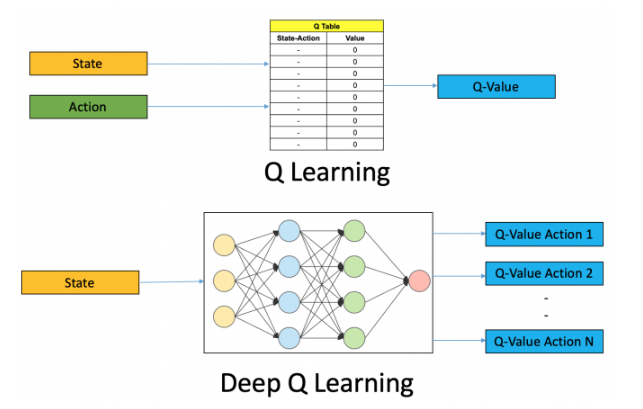
\includegraphics[width=\linewidth]{deepQ}
  \caption{deep Q learning structure \cite{drl}}
  \label{fig:drl}
\end{figure}
\item  \textbf{Find QoS that is required for different applications }
\begin{itemize}
\item \textbf{Bandwidth and throughput}: Bandwidth is the available capacity of connection between two terminals as the most popular term for that is (bps). Throughput slightly differs
from bandwidth as it stands for effective bandwidth that is
provided by network
\item \textbf{Delay or latency:} It specifies the time it takes for a packet
to leave source until reaching the destination. Applications
and network devices can cause delay.
\item \textbf{Jitter (delay variation):} Jitter is an interval between
subsequent packets. It is occurred by network congestion,
route alternation and etc. 
\item \textbf{Loss:} It is amount of packets out of all that are not received
at destination. The success of QOS depends on this factor.
\item \textbf{Reliability:} Some applications are sensitive to packet loss
such as real-time applications. Thus there must be some
mechanism either in application or network to minimize the
packet loss, such as forward error correction (FEC).
\end{itemize}
\begin{figure}%[H]
  \centering
    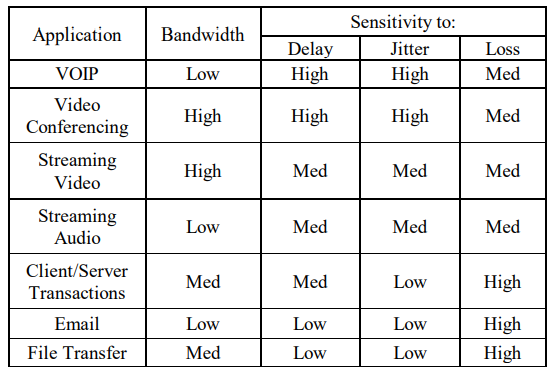
\includegraphics[width=\linewidth]{qos}
  \caption{deep Q learning structure \cite{qos}}
  \label{fig:qos}
\end{figure}
\end{enumerate}

\bibliographystyle{IEEEtran}
\bibliography{references}
\end{document} 